\chapter{THEORY}
\label{THEORY}

The electromagnetic form factors are the fundamental quantities of theoretical and experimental interest as they encode extensive information on the internal structure of the hadron~\cite{Dahiya:2011tv}.
These electromagnetic form factors express the non-local nature of the nucleon in its interactions with photons and have been studied extensively as the basic observables of the nucleon compositeness~\cite{PhysRevLett.95.172503}. 
The increased precision of the electron-proton scattering experiments allowed the extraction of the form factors and using two methods: the Rosenbluth method - also known as the longitudinal-transverse separation technique~\cite{PhysRevD.49.5671,PhysRevD.50.5491,PhysRevLett.94.142301}, and the polarization-transfer technique~\cite{PhysRevLett.84.1398,PhysRevLett.88.092301}.
The two methods show incompatible results when considered in the one-photon exchange approximation, called the Born approximation, to extract the form factors.
It is important to find an explanation of this discrepancy for the use of the electron-proton scattering as a precise and reliable tool in hadronic physics.
Theoretical studies~\cite{PhysRevLett.91.142304,Kondratyuk:2006am} have indicated that the discrepancy could be partially resolved by including higher-order two-photon exchange corrections in the analysis in addition to the lowest-order one-photon exchange approximation.
The calculation in Ref.~\cite{PhysRevLett.91.142304} for the two-photon exchange diagrams considered only nucleons in the intermediate state. 
However, the $\Delta$ resonance has an important role in many hadronic reactions and it is essential to evaluate its contribution to the two-photon exchange in electron-proton scattering.



%The primary goal of the G0 experiment is to measure the parity-violating asymmetries from the elastic scattering of longitudinally-polarized electrons from unpolarized protons in order to use these asymmetries to determine the contribution of strange sea quarks to the charge and magnetization of the nucleon. However, the experiment included the taking of data from which other very interesting and important physics can be extracted about the electromagnetic probe in the elastic scattering of electrons from protons. - Sarah P.

%Several theoretical studies [6,7] have suggested that the problem could be at least partially resolved by including higher-order two-photon exchange corrections in the analysis of electron-proton scattering data, in addition to the lowest-order one-photon exchange (Born) approximation. The recent explicit calculation [6] has shown that with the two-photon exchange taken into account in the analysis of electron-proton scattering, the ratio of the form factors extracted from the LT separation measurements becomes more compatible with the ratio from the PT experiments. However, the two-photon exchange diagrams calculated in Ref. [6] contained only nucleons in the intermediate state; the contribution of other hadrons has not been included until now. In view of the prominent role of the $\Delta$ resonance (unlike other excited states) in many hadronic reactions, it is essential to evaluate its contribution to the two-photon exchange in electron-proton scattering. Without an explicit calculation the results with only the nucleon intermediate state can be viewed only as suggestive in resolving the discrepancy. Some aspects of the $\Delta$ contribution were addressed before [8], using various approximate approaches.

%The electromagnetic form factors reflect the essentially non-local nature of the nucleon in its interactions with photons. As the basic observables par ametrising nucleon compositeness, the form factors have long been studied both experimentally and theoretically. This interest has been renewed recently due to the increased precision of electron-proton scattering experiments and the availability of two alternative methods of extracting the form factors from the data: the Rosenbluth method – also known as the longitudinal-transverse (LT) separation technique [1, 2] – and the polarisation-transfer (PT) technique [3]. If one uses the traditional one-photon exchange calculation to extract the form factors, the two methods lead to apparently incompatible results: while the PT method yields a ratio of the electric to magnetic form factors which falls off linearly with the square of the momentum transfer Q2, the LT separation experiments give an approximately constant ratio [3, 4, 5]. Finding an explanation of this discrepancy is important for the use of electron-proton scattering as a precise and reliable tool in hadronic physics

\begin{figure}[!h]
	\begin{center}
%	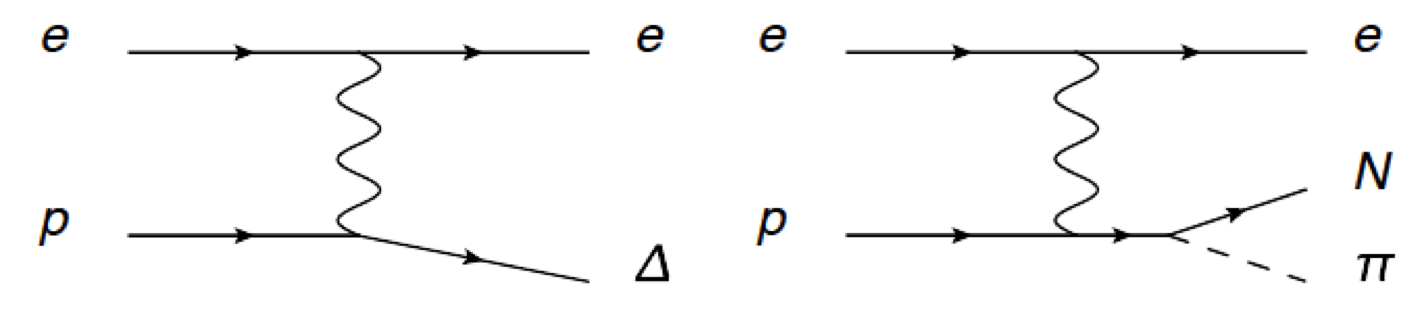
\includegraphics[width=15.0cm]{figures/epeXDeltaCombined}
	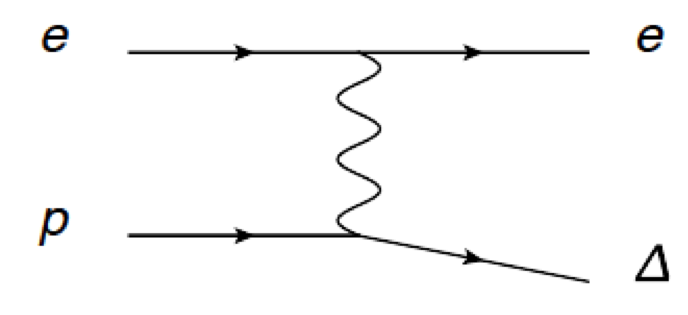
\includegraphics[width=10.0cm]{figures/epeXnoDelta}
	\end{center}
	\caption
%	[Electron-proton $\rightarrow$ electron-$\Delta$ in $\Delta$ region.]
%	{Electron-proton $\rightarrow$ electron-$\Delta$ transition, without and with decay of $\Delta$ in the final state in the one-photon exchange process.}
	{Electron-proton $\rightarrow$ electron-$\Delta$ transition in the one-photon exchange process.}
	\label{fig:epeXDeltaCombined}
\end{figure}

%%%%%%%%%%%%%%%%%%%%%%%%%%%%%%%%%%%%%%%%%%%%%%%%%%%%%%%%%%%%%%%%%%%%%%%
\section{Electron Scattering Beyond the Born Approximation}
\label{Electron Scattering Beyond the Born Approximation}

Beyond the Born approximation, the calculation of the amplitude of the scattering process becomes very complicated. Two or more photons are exchanged in the scattering process and one needs to include all of the excited states of the proton. There are several existing models to calculate multi-photon processes~\cite{Niroula_BornApproximation_thesis}, but they are incomplete.

%
%\subsection{Single Spin Asymmetry in Inelastic Scattering}
%\label{Single Spin Asymmetry in Inelastic Scattering}

%The inelastic contribution is dominated by the region of threshold pion production, as is shown in Fig. 3, where we display the integrand of the W-integration for Bn. When integrating the full curve in Fig. 3 over W, one obtains the total inelastic contribution to Bn (i.e. dashed-dotted curve in Fig. 2).
%
%This contribution at large W mainly drives the results for the inelastic part of the beam asymmetry. Furthermore, it is seen from Fig. 2 that the inelastic and elastic contributions at a low energy of 0.2 GeV have opposite sign, resulting in quite a small asymmetry.
%
%Therefore Bn is a direct measure of the inelastic part which gives rise to sizeable large asymmetries, of the order of several tens of ppm in the backward angular range. At forward angles, the size of the predicted asymmetries is compatible with the first high precision measurements performed at MAMI.
%
%To gain a better understanding of how the inelastic contribution to Bn arises, we show in Fig. 5 the integrand of Bn at Ee = 0.855 GeV and at different scattering angles. The resonance structure is clearly reflected in the integrands for both +n and 0p channels.
%
%In Fig. 6, we show the results for both elastic and inelastic contributions to An at different beam energies.
%
%Going to higher beam energies, the inelastic contribution becomes of comparable magnitude as the elastic one. This is in contrast with the situation for Bn where the elastic contribution already becomes negligible for beam energies around Ee = 0.3 GeV. The integrand of the inelastic contribution at a beam energy of Ee = 0.855 GeV is shown in Fig. 7. The total inelastic result displays a +n threshold region contribution and a peak at the (1232) resonance. Notice that the higher resonance region is suppressed in comparison with the corresponding integrand for Bn. Also the quasi-RCS peak around the maximum W value is absent. As a result, the elastic contribution to An can be of comparable magnitude as the inelastic one. Due to the partial cancellation between elastic and inelastic contributions, An is significantly
%reduced for the proton, taking on values around or below 0.1 \% for beam energies below 1 GeV.

%~\cite{Pasquini2005}


%\subsection{1-photon Exchange in $\Delta$ Region}
%\label{1-photon Exchange in Delta Region}

%For one-photon exchange in $\Delta$ region is not zero, although is proportional to $m_{e}$/$Q$. The asymmetry is proportional to cos$\phi_{\pi}$, the azimuthal angle of the emerging pion relative to the scattering plane. The amplitude can be noted by observing hadronic final state. The variation on $B_{n}$ with scattering angle is shown in Figure~\ref{fig:BNSSA1GammaDelta}~\cite{presentation:CarlCarlson_qweak} by considering only one-photon exchange.


%Considering $\Delta$ as stable state in e+p $\rightarrow$ e+$\Delta$, one can prove the helicity amplitudes are relatively real, and get $B_{n}$ = 0~\cite{presentation:CarlCarlson_qweak}.
%%Treating $\Delta$ as stable, can still prove helicity amplitudes are relatively real, and get $B_{n}$ = 0.
%The $\Delta$ state decays and final state interaction (FSI) gives different phases for different amplitudes. 
%Phases, and whole amplitudes in FSI are known. The multipole amplitudes can be obtained from analyses of other e+p $\rightarrow$ e$\pi$N reactions. 


\begin{figure}[!h]
	\begin{center}
	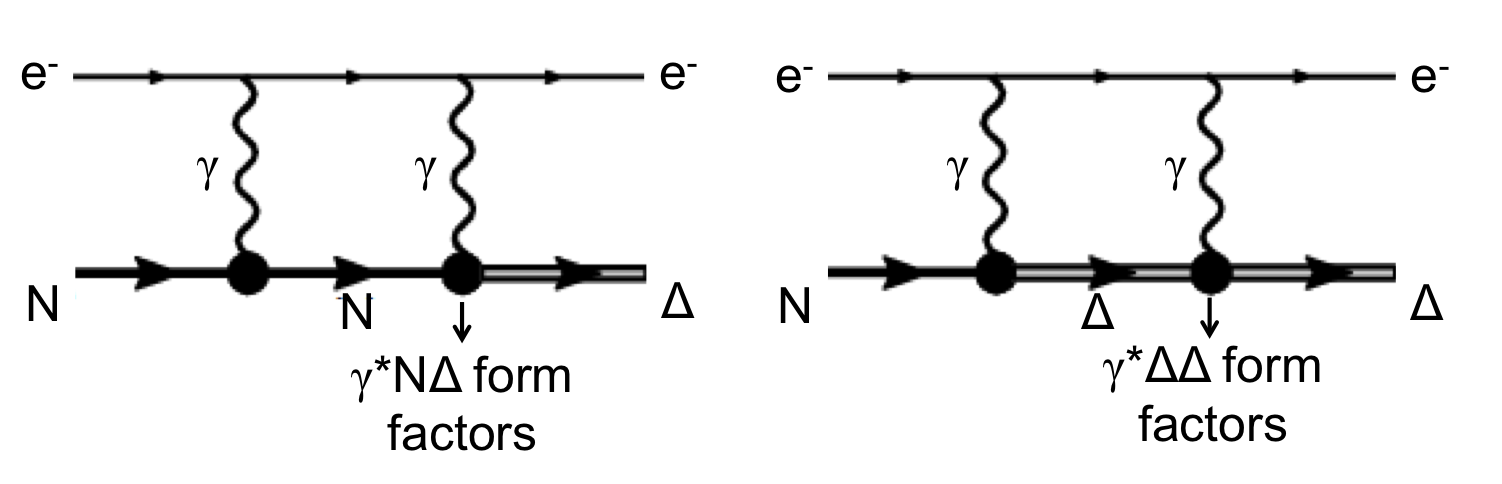
\includegraphics[width=15.0cm]{figures/Im2Gamma}
	\end{center}
	\caption
%	[Transverse Feynman Diagram.]
	{The beam normal single spin asymmetry in inelastic electron-nucleon scattering with $\Delta$ in the final state of the two-photon exchange process. The nucleon as the intermediate state is shown in the left, whereas $\Delta$ as intermediate state is shown in the right.}
	\label{fig:Im2Gamma}
\end{figure}

%%-------------------------------------------------------------------%%
\subsection{Two-photon Exchange}
\label{Two-photon Exchange}

%Apart from the proton’s form-factor ratio, a proper interpretation of the 2-photon exchange process benefits other types of reactions. 
In elastic electron-proton scattering at leading order involves the exchange of a single photon (see Figure~\ref{fig:epeXDeltaCombined}), followed by higher-order processes such as two-photon exchange (as shown in Figure~\ref{fig:Im2Gamma}).
In the Born approximation this is usually approximated as a one-photon. This approximation is possible due to the small value of the electromagnetic coupling constant $\alpha\sim$ 1/137. The higher order processes, such as two-photon exchange, are treated as radiative corrections. The two-photon exchange process involves the exchange of two virtual photons with an intermediate hadronic state that includes the ground state and all the excited states. 
%The two-photon exchange reactions are used to extract information on the hadron structure such as the form factors of the neutron, pion and heavy nuclei (deuteron and $^{3}$He)~\cite{}. 
In the analysis of the form-factor for electron-proton scattering, the contribution of the two-photon exchange amplitude is assumed to be very small~\cite{PhysRev.184.1860}. The real (or dispersive) part of this amplitude is obtained by comparing electron-proton and positron-proton scattering cross sections.
The calculations of the two-photon amplitude can be divided into two categories: unexcited intermediate proton states and excited intermediate proton states. 
The effect of the two-photon exchange contribution with an intermediate $\Delta$ resonance on the elastic electron-proton scattering cross section is smaller in magnitude than the nucleon contribution~\cite{PhysRevLett.95.172503}.

\begin{figure}[h]
	\begin{center}
	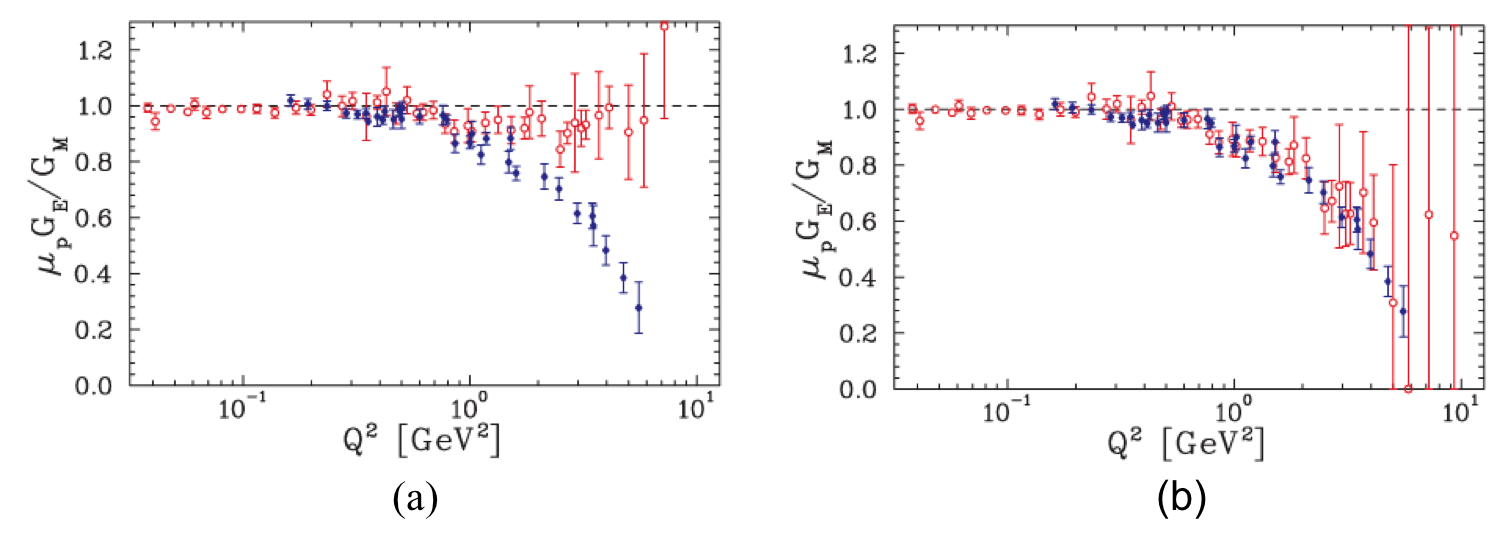
\includegraphics[width=15.0cm]{figures/RosenbluthPolarizationTransfer}
	\end{center}
	\caption
%	[Ratio $\mu_{p}G_{E}/G_{M}$ extracted from the polarization transfer and LT measurements.]
	{Ratio $\mu_{p}G_{E}/G_{M}$ extracted from the polarization transfer (filled diamonds) and LT measurements (open circles). The figure (a) and (b) shows LT separations without and with the two-photon exchange corrections applied to the cross sections, respectively. Figures are from Ref.~\cite{PhysRevC.76.035205}.}
	\label{fig:RosenbluthPolarizationTransfer}
\end{figure}

The first experimental evidence for the importance of the proper treatment of the two-photon exchange was seen with the measurement~\cite{PhysRevLett.84.1398} of the proton’s electric ($G_{E}$) and magnetic form factor ($G_{M}$) ratio using the polarization transfer technique~\cite{PhysRevC.23.363}. This is a complementary measurement to the Rosenbluth separation technique~\cite{PhysRev.79.615}.
%This measurement, which is complementary to the Rosenbluth separation technique~\cite{PhysRev.79.615}, yielded a GE/GM ratio which deviated from the Rosenbluth results at Q2 above 1 (GeV/c)2.
The discrepancy in the form factors extracted between the Rosenbluth separation and the polarization transfer techniques using the one-photon exchange approximation is shown in Figure~\ref{fig:RosenbluthPolarizationTransfer} (a)~\cite{PhysRevC.76.035205}. The form factor results start to deviate above $Q^{2}$ of 1~(GeV/c)$^{2}$. After applying the two-photon exchange correction, the discrepancy seems to be resolved between the two methods, as shown in Figure~\ref{fig:RosenbluthPolarizationTransfer} (b)~\cite{PhysRevC.76.035205}.
The two-photon exchange calculations are not complete and have not been tested over a wider range of kinematics.

Another question naturally arises whether other higher-mass resonances could also have a non-negligible contribution to the two-photon exchange correction such as the $\Delta$(1232) resonance~\cite{Arrington2011782}. The effects turn out to be not too important, as shown by Kondratyuk and Blunden~\cite{PhysRevC.75.038201} by generalizing the calculation to full spectrum of the most important hadron resonances as intermediate states involving spin 1/2 and 3/2 resonances.

%If the $\Delta$(1232) resonance makes a non-negligible contribution to the TPE correction, at least in some kinematic regions, the question naturally arises whether other, higher-mass resonances could also play some role. Kondratyuk and Blunden [102] extended the formalism of Refs. [5, 7], generalizing it to include the full spectrum of the most important hadron resonances as intermediate states involving spin 1/2 and 3/2 resonances. The masses of the resonances and their nucleon-photon coupling constants are based on dynamical multichannel calculations [99, 103, 104] of nucleon Compton scattering at low and intermediate energies. The resonance TPE effects turn out to be not too sensitive to the details of these models.~\cite{Arrington2011782}


%%%%%%%%%%%%%%%%%%%%%%%%%%%%%%%%%%%%%%%%%%%%%%%%%%%%%%%%%%%%%%%%%%%%%%%
\section{Experimental Observation of Beam Spin Asymmetry}
\label{Experimental Observation of Beam Spin Asymmetry}

The beam spin asymmetries are time-reversal odd, parity conserving observables which vanish in the Born approximation. The beam spin asymmetry is an observable of the imaginary part of the two-photon exchange amplitude and can be extracted by observing only the electron (as shown in Figures~\ref{fig:epeXDeltaCombined} and \ref{fig:Im2Gamma}). The asymmetry arises from the interference of the imaginary part of the two-photon exchange and one-photon exchange amplitude. Since the one-photon amplitude is real, only the imaginary part of the two-photon amplitude contributes to the beam spin asymmetry. The asymmetry is due to an electron helicity flip. 
The asymmetry can be obtained either by polarizing the target perpendicular (transverse) to the incoming unpolarized electron beam, or by a transversely polarized beam on an unpolarized target. 
The asymmetry in the first case is known as target normal single spin asymmetry ($A_{n}$) while the latter case is called the beam normal single spin asymmetry ($B_{n}$). The measured asymmetry can be expressed as 

%where the measured asymmetry ($A_{M}$) has a sinusoidal dependence about the beam axis
%
%The asymmetries in the latter case are called beam normal single spin asymmetries ($B_{n}$) where the measured asymmetry ($A_{M}$) has a sinusoidal dependence about the beam axis
\begin{equation} \label{equ:transverse20}
\epsilon_{M} = \frac{\sigma^{\uparrow} - \sigma^{\downarrow} }{\sigma^{\uparrow} + \sigma^{\downarrow}} = \frac{\Im \left[ \sum\limits_{spins} (\mathcal{M}^{\gamma})^{*}(Abs\mathcal{M}^{\gamma\gamma}) \right] }{\sum\limits_{spins} |\mathcal{M}^{\gamma}|^{2} },
\end{equation}

\noindent
where $\sigma^{\uparrow,\downarrow}$ are cross sections with incoming electrons polarized up or down, perpendicular to the scattering plane. Here, $\Im$ is the imaginary part and $Abs\mathcal{M}^{\gamma\gamma}$ is a sum over all the possible intermediate states in the two-photon exchange
process. 
The cross section can be parameterized using six invariant amplitudes $\tilde{G}_{E}(\nu,Q^{2})$ , $\tilde{G}_{M}(\nu,Q^{2})$, and $\tilde{F}_{i}(\nu,Q^{2})$, which are complex functions of the $Q^{2}$ and $\nu$. Here $\nu$ = $K \cdot P$, where K and P are the average of the incoming electron and outgoing proton four-momenta, respectively~\cite{Gorchtein2005273, juliette_G0_thesis}.
In the Born approximation, the complex electromagnetic form factors become the usual Pauli and Sachs form factors of the nucleon, 
$\tilde{G}_{E}(\nu,Q^{2}) \rightarrow G_{E}(Q^{2})$, $\tilde{G}_{M}(\nu,Q^{2}) \rightarrow G_{M}(Q^{2})$, and $\tilde{F}_{i}(\nu,Q^{2}) \rightarrow 0$. 
Since $\tilde{F}_{i}$ and the phases of $\tilde{G}_{E}$ and $\tilde{G}_{E}$ vanish in the Born approximation, they must originate from processes involving at least the exchange of two photons. 
After Born approximation, using this parameterization, with the virtual photon polarization parameter, 

\begin{equation} \label{equ:transverse16}
\varepsilon = \frac{\nu^{2} - M^{4}\tau( 1 + \tau )}{\nu^{2} + M^{4}\tau( 1 + \tau )}, 
\end{equation}

\noindent
the beam normal single spin asymmetry can be expressed as~\cite{Gorchtein2004234}

\begin{dmath}
%\begin{equation} \label{equ:transverse22}
B_{n} = \frac{2m_{e}}{Q} \sqrt{2\varepsilon(1-\varepsilon)} \sqrt{1+\frac{1}{\tau}} \left( G_{M}^{2} + \frac{\varepsilon}{\tau}G_{E}^{2} \right)^{-1} \times \left[ - \tau G_{M} \Im \left( \tilde{F}_{3} + \frac{1}{1+\tau} \frac{\nu}{M^{2}} \tilde{F}_{5} \right) - G_{E}\Im \left( \tilde{F}_{4} + \frac{1}{1+\tau} \frac{\nu}{M^{2}} \tilde{F}_{5} \right) \right] + \mathcal{O}(e^{4}),
%\end{equation}
\end{dmath}

\noindent
whereas the target normal spin asymmetry can be written as

\begin{dmath}
%\begin{equation} \label{equ:transverse21}
A_{n} = \sqrt{\frac{1\varepsilon(1+\varepsilon)}{\tau}} \left( G_{M}^{2} + \frac{\varepsilon}{\tau}G_{E}^{2} \right)^{-1} \times \left[ -G_{M} \Im \left( \delta\tilde{G}_{E} + \frac{\nu}{M^{2}}\tilde{F}_{3} \right) + G_{E}\Im \left( \delta \tilde{G}_{M} + \frac{2\varepsilon}{1+\varepsilon} \frac{\nu}{M^{2}} \tilde{F}_{3} \right) \right] + \mathcal{O}(e^{4}).
%\end{equation}
\end{dmath}

\noindent
An ultra-relativistic particle can be polarized in the direction normal to its momentum with a suppression factor $m$/$E$, where $m$ is the mass and $E$ is the energy of the particle~\cite{doi:10.1146/annurev.nucl.57.090506.123116}. 
%To polarize an ultra-relativistic particle in the direction normal to its momentum involves a suppression factor $m$/$E$, where $m$ is the mass and $E$ is the energy of the particle~\cite{doi:10.1146/annurev.nucl.57.090506.123116}. 
The suppression factor for the electron with beam energy in the 1~GeV range is of order $10^{-4}$ to $10^{-3}$. The resulting beam normal single spin asymmetry is expected to be of order $10^{-6}$ to $10^{-5}$, whereas the target-normal spin asymmetry is of order $10^{-2}$~\cite{doi:10.1146/annurev.nucl.57.090506.123116}.


%Furthermore, to polarize an ultrarelativistic
%particle in the direction normal to its momentum involves a suppression factor m/E
%(with m the mass and E the energy of the particle), which for the electron is of
%order 10−4−10−3 when the electron beam energy is in the 1-GeV range. Therefore,
%the resulting target-normal SSA is expected to be of order 10−2, whereas the beamnormal
%SSA is of order 10−6−10−5. A measurement of such small asymmetries is
%quite demanding experimentally. However, in the case of a polarized lepton beam,
%asymmetries of the order of parts per million are currently accessible in PV elastic
%eN scattering experiments. The PV asymmetry involves a beam spin polarized along
%its momentum. However, the SSA for an electron beam spin normal to the scattering
%plane can also be measured using the same experimental setups. First measurements
%of this beam-normal SSA at beam energies up to 1 GeV have yielded values near
%−10 ppm (95–97) in the forward angular range and up to an order of magnitude
%larger in the backward angular range (98). At higher beam energies, first results for
%the beam-normal SSA in elastic eN scattering experiments were also reported recently
%(97, 99, 100).


%where terms of order 2 and higher are neglected. There is an order me=E suppression in
%addition to the factor of  leading to asymmetries on the order of 10􀀀6 􀀀 10􀀀5. Thus the
%techniques developed for measuring the small parity-violating asymmetries are also useful
%for measuring these asymmetries.

%Beam normal single spin asymmetries are generated by the interference of the one-photon and two-photon exchange processes~\cite{DeRujula1971365} for e-p $\rightarrow$ e-X in the $\Delta$ region is given by 
%%Beam spin asymmetry for ep $\rightarrow$ eX in the $\Delta$ region is given by
%
%\begin{equation} \label{equ:transverseElastic}
%B_{n} = \frac{\sigma^{\uparrow} - \sigma^{\downarrow} }{\sigma^{\uparrow} + \sigma^{\downarrow}} = \frac{2\Im \left( M_{+}M_{-}^{*} \right) }{ |M_{+}|^{2} + |M_{-}|^{2} }.
%\end{equation}
%
%%where $\sigma^{\uparrow,\downarrow}$ are cross sections with incoming electrons polarized up or down, perpendicular to the scattering plane. 
%$M_{\pm}$ are helicity amplitudes, with incoming electrons polarized parallel or anti-parallel to momentum. The asymmetries are time-reversal invariant, and parity conserving observables which vanish in the Born approximation. In the one photon exchange approximation for elastic scattering, all helicity amplitudes are relatively real, and $B_{n}$(elastic,1$\gamma$) = 0.

%The beam normal single spin asymmetry (BNSSA) is a parity-conserving asymmetry that arises due to the interference of two photon exchange with that of a single photon~\cite{PhysRevC.70.045206}, and is also known as transverse asymmetry. BNSSA is generated by the scattering of polarized electrons from unpolarized protons is a possible false background asymmetry in parity violating electron scattering experiments (PVES). 
%%There is a parity conserving Beam Normal Single Spin Asymmetry or transverse asymmetry (An) on H2 with a sin(φ)-like dependence due to 2-γ exchange. 
%The size of $B_{n}$ is few ppm, so a few percent residual transverse polarization in the beam, in addition to potentially small broken azimuthal symmetries in the detector, might lead to few ppb corrections to the Q-weak data. As part of a program of $B_{n}$ background studies, we made the first measurement of $B_{n}$ in the N-to-Delta transition using the Q-weak apparatus. $B_{n}$ from electron-nucleon scattering is also a unique tool to study the $\gamma^{*}\Delta\Delta$ form factors~\cite{Alexandrou2009115}.
%Studying the nonlinearity of the two-photon exchange contribution for the $\Delta$ production process~\cite{PhysRevC.73.025206} may help to obtain additional information on the $\gamma^{*}\Delta\Delta$ coupling constant, which is a scarcely known but much needed ingredient in nuclear physics (such as studies of isobar contributions to the deuteron wave function)~\cite{Kondratyuk:2006am}.
%
%
%If the transverse asymmetry is measured at energies below or around the two-pion production
%threshold, the electroproduction amplitudes used in the calculations of the intermediate states are
%relatively well known, since pion electroproduction experiments can be used as input. Conversely,
%as the transverse asymmetry is sensitive to the electroproduction amplitudes on the nucleon, the
%asymmetry could provide information on resonance transition form factors.
%Pasquini and Vanderhaeghen [140] used this method to calculate the imaginary part of the
%two-photon exchange amplitude, by relating the amplitude to the contribution of X = N and X =
%πN intermediate state contributions through unitarity. The πN intermediate state contributions
%were assessed using the phenomenological MAID analysis [155] to obtain the corresponding pion
%electroproduction amplitudes. Both resonant and non-resonant pion production mechanisms are
%included in the MAID analysis. The results of the calculation show that at forward angles, the
%quasi-real Compton scattering at the endpoint W = Wmax only yields a very small contribution.
%However, it grows larger going to backward angles, because the quasi-real Compton scattering
%contribution is the opposite sign as the remainder of the integrand, which determines the location
%of the absolute maximum value of the transverse asymmetry.
%
%The results for the full calculation (solid line) of An are shown in Figure 2.10 for beam energies
%of 0.3, 0.424, 0.570, and 0.855 GeV, along with the results for only the nucleon intermediate state
%(the dashed line) and the πN inelastic contribution (dashed-dotted line). At these energies, the
%nucleon intermediate state has a relatively small contribution compared to the inelastic states,
%making An primarily a measure of the inelastic part. The transverse asymmetries are large in
%the backward-angle region, because of the quasi-real Compton scattering near singularity. The
%transverse asymmetry has been measured in this energy region by the A4 collaboration (see Section
%3.4.2). At forward angles, the predicted asymmetries are compatible, although the calculation
%somewhat overpredicts the absolute size of the asymmetry in this range [156]. However, asymmetries
%of this size (∼ 100 ppm around θCM = 150◦) in the backward-angle range have recently been
%observed in preliminary results by the A4 collaboration [157]. More backward-angle transverse
%asymmetry data has also recently been taken by the G0 collaboration in this energy region (see
%Section 7.1.2).

%It is noteworthy that by studying the nonlinearity
%of the two-photon exchange contribution for the A production process [4] one may be
%able to obtain additional information on the yAA coupling constant, a scarcely known
%but much needed ingredient in nuclear physics (such as studies of isobar contributions
%to the deuteron wave function).

\begin{singlespace}
\begin{figure}[!h]
	\begin{center}
	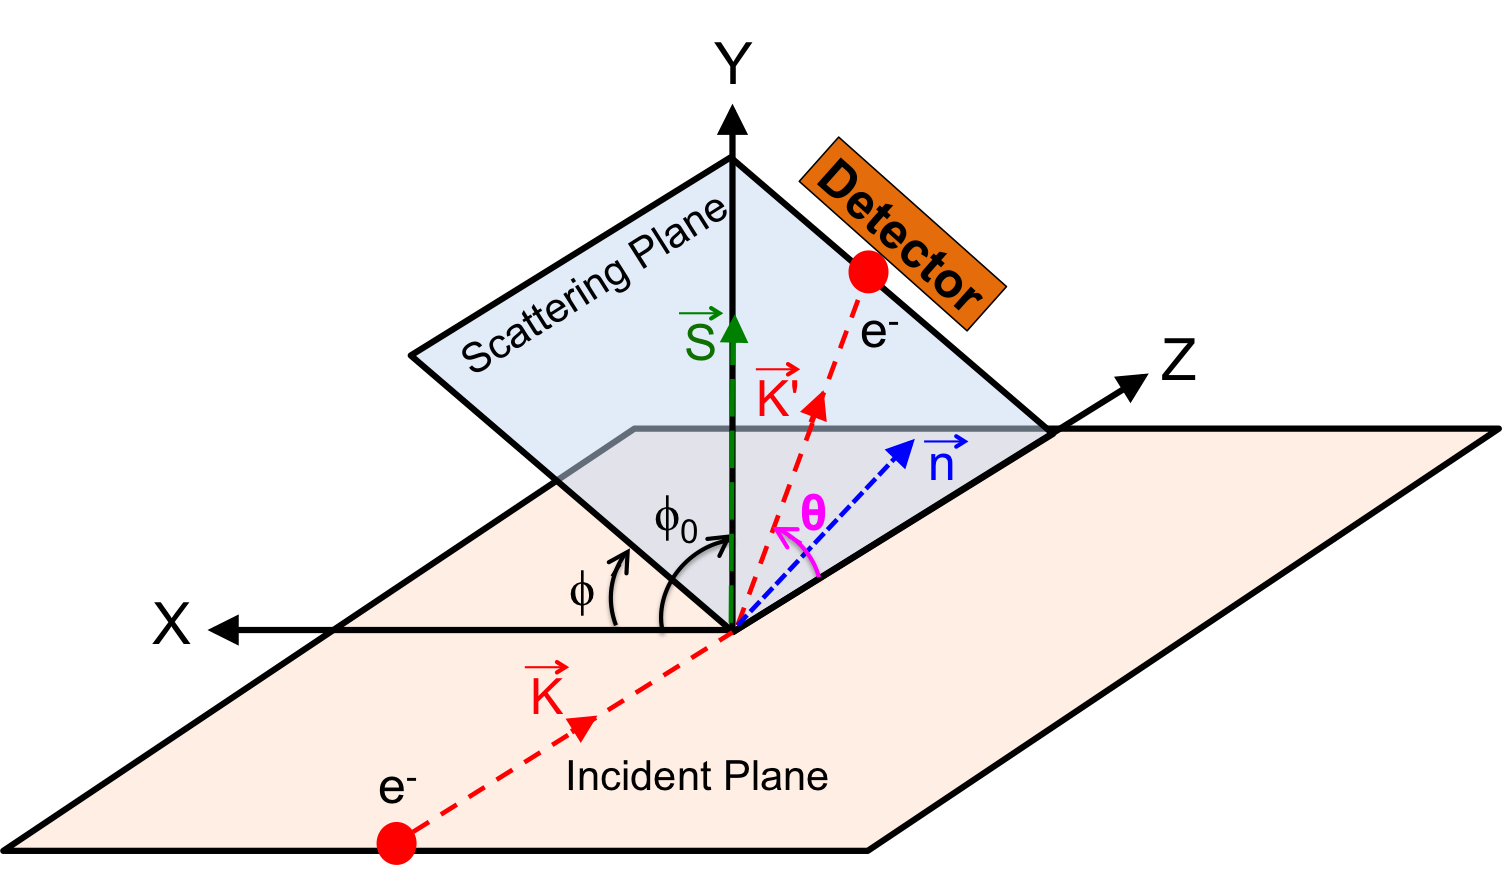
\includegraphics[width=15.0cm]{figures/transverse_diagram}
	\end{center}
	\caption
%	[The schematic of transverse electron-nucleon scattering reaction.]
	{The schematic of transverse electron-nucleon scattering reaction. The electron spin is polarized in the vertical transverse direction. The initial (final) momentum of the electron is given by $\vec{K}$ ($\vec{K}^{\prime}$).}
	\label{fig:transverse_diagram}
\end{figure}
\end{singlespace}

%%-------------------------------------------------------------------%%
\subsection{Measurement of the Beam Normal Single Spin Asymmetry}
\label{Measurement of the Beam Normal Single Spin Asymmetry}

The beam normal single spin asymmetry (BNSSA) is measured by scattering transversely polarized electrons from unpolarized nucleons. The measured asymmetry ($\epsilon_{M}$) has a sinusoidal dependence about the beam axis 

\begin{equation} \label{equ:transverse1}
\epsilon_{M} (\phi) = - B_{n} \vec{S} \cdot \hat{n} = - B_{n} |\vec{S}| \sin (\phi-\phi_{0}),
\end{equation}

\noindent
where $\vec{S}$ is the electron spin in the transverse direction, and $\hat{n}$ is the unit vector normal to the scattering plane (see Figure~\ref{fig:transverse_diagram}). Here, $\phi_{0}$ and $\phi$ are the azimuthal angles of $\vec{S}$ and the scattering plane, respectively with respect to incident plane. 
%The beam normal single spin asymmetry can be measured and extracted from the asymmetry measured in the detector placed at azimuthal angle $\phi$.
The beam normal single spin asymmetry can be measured and extracted from the asymmetry measured in the detectors placed at fixed scattering angle $\theta$ along the azimuthal angle $\phi$.

%Put the final state interaction on the electron side, therefore just observing electron can give Beam Spin Asymmetry.
%Put the final state interaction on the electron side, whence just observing electron can give Beam Spin Asymmetry. Figure~\ref{fig:transverseFeynmanDiagram}.
%Since 1$\gamma$ amplitude real, only need Im part of 2$\gamma$ amplitude. And,


\begin{singlespace}
\begin{figure}[!h]
	\begin{center}
	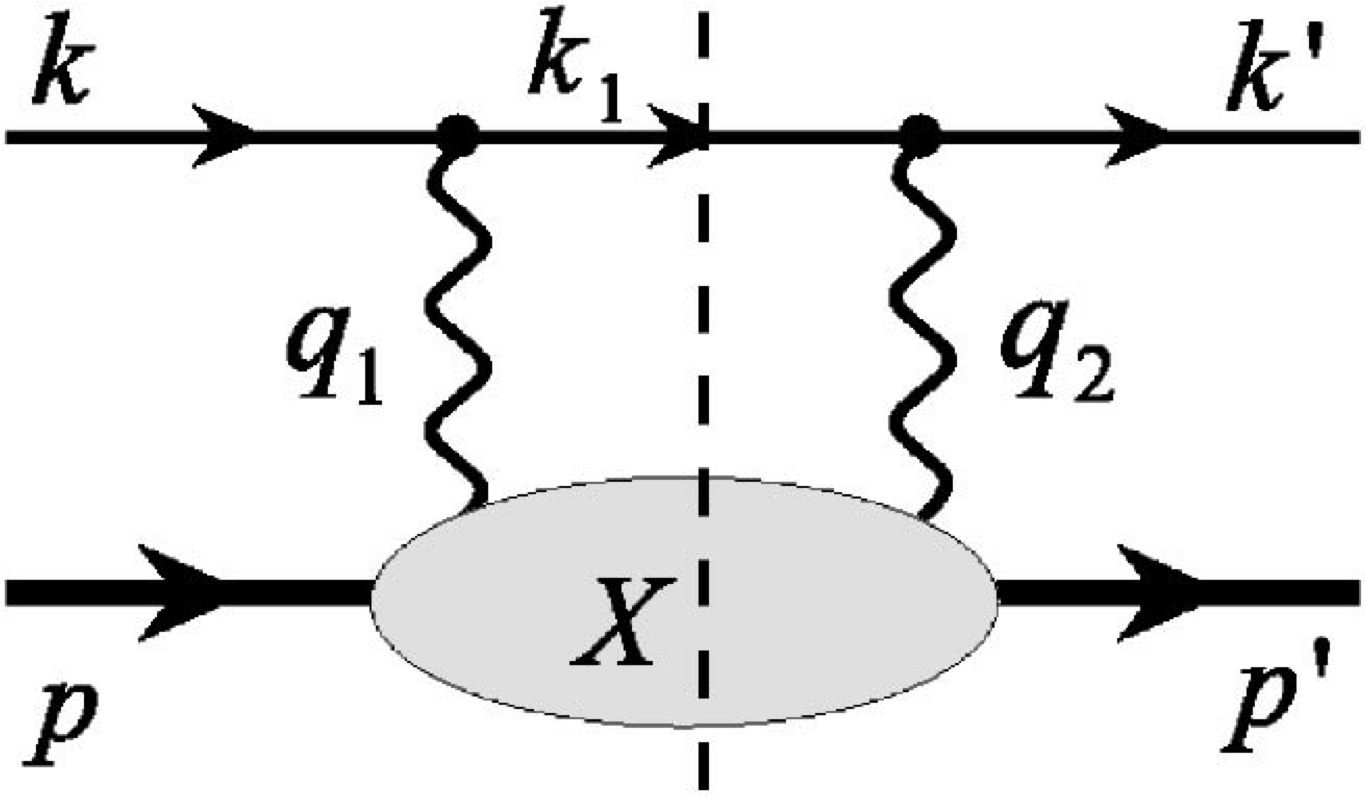
\includegraphics[width=8.0cm]{figures/FeynmanDiagrams_ep}
	\end{center}
	\caption
%	[The two-photon exchange diagram. The filled blob represents the response of the nucleon to the scattering of the virtual photon.]
	{The two-photon exchange diagram. The filled blob represents the response of the nucleon to the scattering of the virtual photon~\cite{PhysRevC.70.045206, Pasquini2005}.}
	\label{fig:FeynmanDiagrams_ep}
\end{figure}
\end{singlespace}


%%-------------------------------------------------------------------%%
\subsection{Imaginary Part of Two-photon Diagram}

The imaginary part of the two-photon exchange amplitude is related to the absorptive part of the doubly virtual Compton scattering (DVCS) amplitude on the nucleon, as shown in Figure~\ref{fig:FeynmanDiagrams_ep} and can be written as~\cite{PhysRevC.73.055201}

\begin{equation} \label{equ:transverse23}
Abs \mathcal{M}^{\gamma\gamma} = e^{4} \int \frac{ |\vec{k}_{1}|^{2} d|\vec{k}_{1}| d\Omega_{k_{1}} }{2E_{k_{1}}(2\pi)^{3}} \bar{u}(k^{\prime}) \gamma_{\mu}(\gamma k_{1} + m_{e}) \gamma_{\nu} u(k) \frac{1}{Q_{1}^{2} Q_{2}^{2}} W^{\mu\nu}(w, Q_{1}^{2}, Q_{2}^{2})
\end{equation}


The inelastic contribution to $W^{\mu\nu}$ corresponding with the $\pi$N intermediate states in the blob of Figure~\ref{fig:FeynmanDiagrams_ep}\footnote{can be calculated using the MAID model (resonance region)}~\cite{PhysRevC.73.055201} is given by

\begin{dmath}
%\begin{equation} 
\label{equ:transverse24}
W^{\mu\nu} (p^{\prime}, \lambda_N^{\prime}; p, \lambda_N) = \frac{1}{4\pi^{2}} \frac{ |\vec{p}_{\pi}|^{2}}{[ |\vec{p}_{\pi}| (E_{\pi} + E_{n}) + E_{\pi}|\vec{k}_{1}|\hat{k}_{1}\cdot\hat{p}_{\pi}]} \times \sum_{\lambda_{n}} \int d\Omega_{\pi}\bar{u}(p^{\prime},\lambda_{N}^{\prime}) J_{\pi N}^{\dagger\mu} u (p_{n},\lambda_{n}) \times \bar{u}(p_{n},\lambda_{n}) J_{\pi N}^{\nu} u (p,\lambda_{N})
%\end{equation}
\end{dmath}

\noindent
where $p_{\pi} = (E_{\pi},\vec{p}_{\pi})$ and $p_{n} = (E_{n},\vec{p}_{n})$ are the four-momenta of the intermediate pion and nucleon states, respectively, and $k_{1} = - \vec{p}_{\pi} - \vec{p}_{n}$. The integration runs over the polar and azimuthal angles of the intermediate pion, and $J_{\pi N}^{\nu}$ and $J_{\pi N}^{\dagger\mu}$ are the pion electro-production currents, describing the excitation and deexcitation of the $\pi N$ intermediate state, respectively. $u$ and $\bar{u}$ are matrix elements and can be parameterized. The inelastic contribution is dominated by the region of pion production threshold.


%%%%%%%%%%%%%%%%%%%%%%%%%%%%%%%%%%%%%%%%%%%%%%%%%%%%%%%%%%%%%%%%%%%%%%%
\section{The $\gamma^{*}\Delta\Delta$ Form Factors}

%Intermediate hadrons are on-shell.
The proton electromagnetic form factor is well known, experimentally. The proton $\rightarrow \Delta$ electromagnetic transition form factor is also fairly well known. 
For proton and $\Delta$ intermediate hadrons, vertices therefore are known except for the $\gamma^{*}\Delta\Delta$ electromagnetic vertex.
%The only missing information is about $\gamma^{*}\Delta\Delta$ form factor. 
The information about the $\gamma^{*}\Delta\Delta$ form factor has the potential to measure the charge radius of $\Delta$ and magnetic moment of $\Delta$. Besides there have been many theoretical interest: 
%$\gamma\Delta\Delta$ form factors have been of theoretical interest:
\begin{itemize}
\item Dyson-Schwinger approach~\cite{Segovia2014}
\item Covariant quark model~\cite{PhysRevD.86.093022}
\item Lattice QCD~\cite{Alexandrou2009115}
\end{itemize}

%\item Dyson-Schwinger approach (Segovia et al., 2013)
%\item Covariant quark model (Ramalho et al., 2010)~\cite{PhysRevD.86.093022}
%\item Lattice QCD (Alexandrou et al., 2009)~\cite{Alexandrou2009115}


This form factor has never been measured before. 
No dedicated calculations exist to relate $\gamma^{*}\Delta\Delta$ form factors to cross section or asymmetry data.


%%%%%%%%%%%%%%%%%%%%%%%%%%%%%%%%%%%%%%%%%%%%%%%%%%%%%%%%%%%%%%%%%%%%%%%
\section{Model Calculations}
\label{Model Calculations}

\begin{figure}[!h]
	\begin{center}
	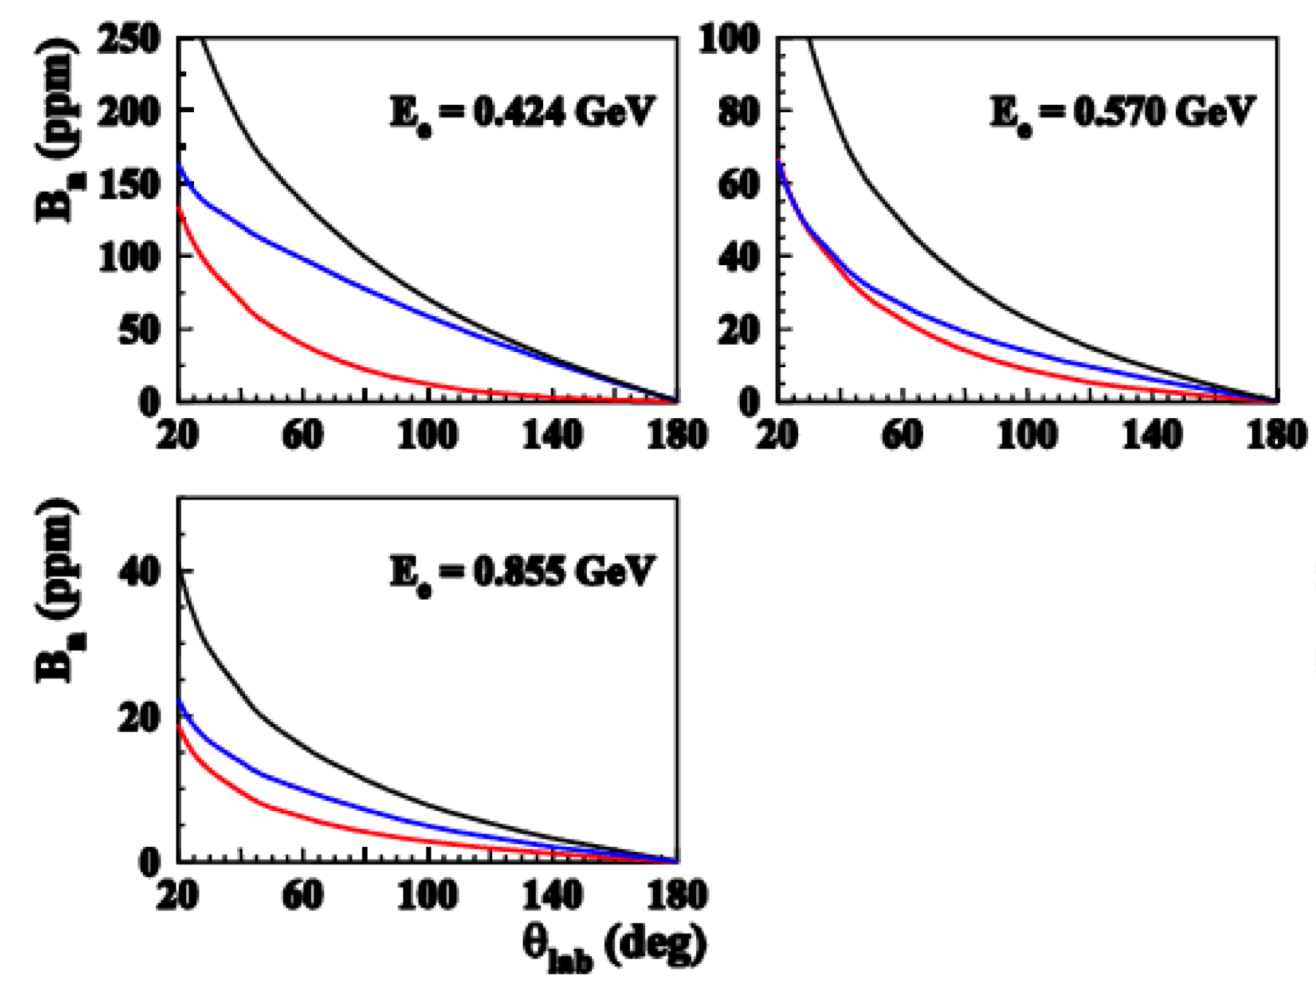
\includegraphics[width=15.0cm]{figures/PasquiniInelasticTransverseAsymmetryModel}
	\end{center}
	\caption
%	[Inelastic transverse asymmetry model from Pasquini et al.]	
	{Inelastic transverse asymmetry model from Pasquini et al.~\cite{presentation:pasquini_Mainz}. $\Delta$ intermediate state is shown in red, N intermediate state is shown in blue, and total ($\Delta$+N) contribution is shown in black.}
	\label{fig:PasquiniInelasticTransverseAsymmetryModel}
\end{figure}


The only model calculation of the beam normal single spin asymmetry in inelastic electron-nucleon scattering was performed (unpublished) by Pasquini \& Vanderhaeghen for forward angles and low energies~\cite{presentation:pasquini_Mainz, presentation:CarlCarlson_qweak}. The BNSSA as a function of the center-of-mass angle, $\theta_{cm}$, for $\Delta$ (red) and nucleon (blue) intermediate states is shown in Figure~\ref{fig:PasquiniInelasticTransverseAsymmetryModel}. If the intermediate hadronic states are not included in the calculation, the prediction is nearly flat as a function of the $\theta_{cm}$. This calculation was performed for lower energy than Q-weak, and an effort to extrapolate this result to the Q-weak kinematic settings is discussed in chapter~\ref{BEAM NORMAL SINGLE SPIN ASYMMETRY}. The beam normal single spin asymmetry is positive and of the order of 50~ppm. The large asymmetries in the forward region are dominated by quasi-virtual Compton scattering kinematics, where one exchanged photon becomes quasi-real. The asymmetry almost exponentially varies with scattering angle. 

%\begin{figure}[h]
%	\begin{center}
%	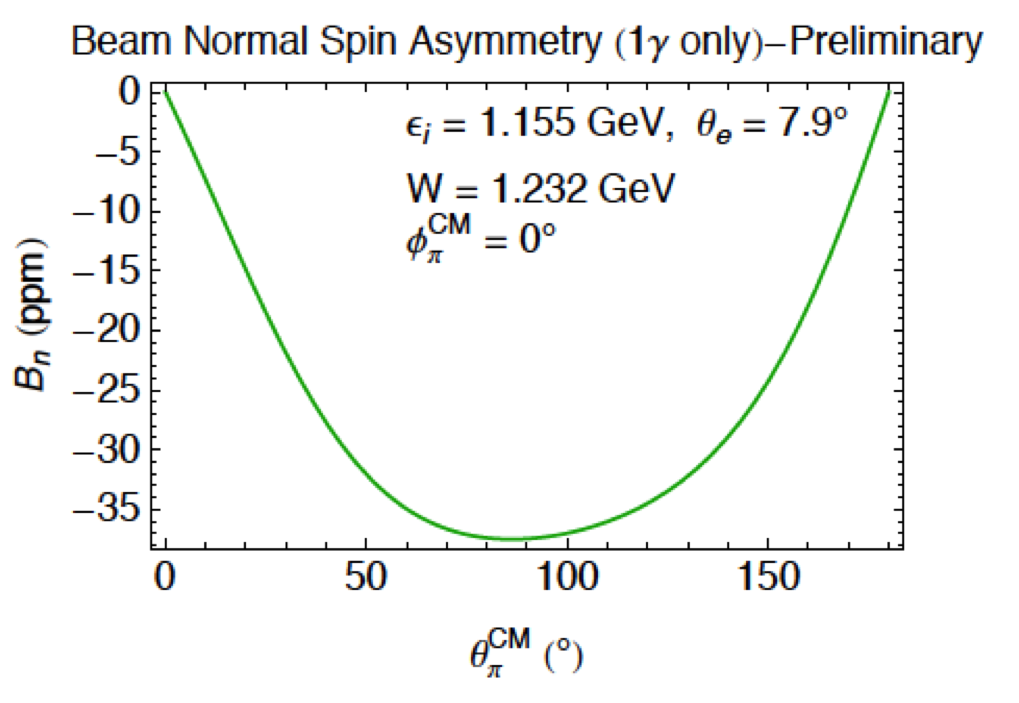
\includegraphics[width=12.0cm]{figures/BNSSA1GammaDelta}
%	\end{center}
%	\caption
%	[Beam normal single spin asymmetry with decay of $\Delta$ in the final state for one-photon exchange.]
%	{Beam normal single spin asymmetry with decay of $\Delta$ in the final state for one-photon exchange.}
%	\label{fig:BNSSA1GammaDelta}
%\end{figure}
%
%There is an ongoing calculation for one-photon exchange in $\Delta$ region~\cite{presentation:CarlCarlson_qweak}, which shows the beam normal spin asymmetry is not zero, although it is proportional to $m_{e}$/$Q$. The asymmetry is proportional to cos$\phi_{\pi}$, the azimuthal angle of the emerging pion relative to the scattering plane. 
%Considering $\Delta$ as stable state in e+p $\rightarrow$ e+$\Delta$, one can prove the helicity amplitudes are relatively real, and get $B_{n}$ = 0~\cite{presentation:CarlCarlson_qweak}.
%The $\Delta$ state decays and final state interaction (FSI) gives different phases for different amplitudes. 
%The phases, and whole amplitudes in FSI are known. The multipole amplitudes can be obtained from analyses of other e+p $\rightarrow$ e$\pi$N reactions and observing hadronic final state.
%%The amplitude can be noted by observing hadronic final state. 
%The variation on $B_{n}$ with scattering angle is shown in Figure~\ref{fig:BNSSA1GammaDelta}~\cite{presentation:CarlCarlson_qweak} by considering only one-photon exchange.


%%%%%%%%%%%%%%%%%%%%%%%%%%%%%%%%%%%%%%%%%%%%%%%%%%%%%%%%%%%%%%%%%%%%%%%
\section{Goals of the Inelastic Transverse Physics Program}

The objective of the Q-weak experiment is to challenge the predictions of the Standard Model in low $Q^{2}$ range and search for new physics at the TeV scale through a 4\% measurement of the weak charge of the proton via the parity-violating asymmetry ($\sim$250~ppb) in elastic e+p scattering~\cite{qweak_proposal_2007}. There is a parity conserving beam normal single spin asymmetry, or transverse asymmetry, $B_{n}$ on H$_{2}$ with a sin($\phi$)-like dependence due to the two-photon exchange. The expected magnitude of $B_{n}$ is few ppm which is an order of magnitude larger than PV asymmetry for the Q-weak and may produce a small background. 
Also $B_{n}$ provides direct access to the imaginary part of the two-photon exchange amplitude. It will be interesting to see the magnitude of $B_{n}$ in the N$\rightarrow\Delta$ region which has never been measured before. 
$B_{n}$ from electron-nucleon scattering is also a unique tool to study the $\gamma^{*}\Delta\Delta$ form factors. 
This dissertation presents the analysis of the 9\% measurement of the beam normal single spin asymmetry in inelastic electron-proton scattering at a $Q^{2}$ of 0.0209 (GeV/c)$^{2}$. This measurement will help to improve the theoretical models on the beam normal single spin asymmetry and thereby our understanding of the doubly virtual Compton scattering process.


%\begin{equation} \label{equ:transverseDef1}
%A_{M} = \frac{\Im  (T^{\gamma})^{*}(AbsT^{\gamma\gamma})  }{|T^{\gamma}|^{2} }
%\end{equation}
%
%
%\cite{PhysRevLett.96.012301}
%
%From ELOG: \url{https://qweak.jlab.org/elog/Analysis+\%26+Simulation/410}
%
%\begin{equation} \label{equ:transverse1}
%A_{M}  (\phi) = - B_{n} *[ P^{V} \cos(\phi) - P^{H} \sin(\phi) ]
%\end{equation}
%
%with 
%$B_{n}$ the analyzing power and 
%$P^{V}$ = P $\sin$($\theta_{s}$) $\sin$($\phi_{s}$)
%$P^{H}$ = P $\sin$($\theta_{s}$) $\sin$($\phi_{s}$)
%
%This leads to 
%\begin{equation} \label{equ:transverse2}
% A^{V}_{M} = - B_{n} P \cos(\phi); \quad  A^{H}_{M} = - B_{n} P \sin(\phi)
%\end{equation}
%
%when beam is vertically transverse polarized ($P^V$ $\rightarrow$ $P$) and when the beam is horizontally transverse polarized ($P^H$ $\rightarrow$ $P$).
%
%\begin{equation} \label{equ:transverse3}
%A = (A^{V}_{M})*[p_{0} \cos(\phi) - p_{1} \sin(\phi)]  + p_{2}
%\end{equation}
%
%where  $A_{Vm}$  is measured  vertical transverse asymmetry from transverse data, $A_{VT}$ = -4.75 ppm 
%and $\phi$ is the azimuthal angle. $\phi$ = 0 is octant 1 and so on.
%
%Note:  
%In a given octant during vertical transverse running
%	$A_{Vm}$ = $P$ * $B_{n}$     
%	and during longitudinal running
%      	$A_{mV}$ =  $P_{V}$ * $B_{n}$
%	So we can write 
%      	$A_{mV}$ = $A_{Vm}$ *($P_{V}$/$P$)
%	with ($P_{T}$/$P$) giving the fraction of vertical transverse polarization present in the beam.
%Similarly we can use  $P_{H}$/$P$ to get the fraction of horizontal traverse polarization in the beam.
%
%Therefore, in the fit,
%
%   $p_{0}$  = ($P^{V}$/$P$)  fraction of vertical transverse polarization in the beam
%   $p_{1}$  = ($P^{H}$/$P$)  fraction of vertical horizontal polarization in the beam
%   $p_{2}$  =  $P^{L}$*$A_{PV}$ + other false asymmetries (if there is any).
%
%
%\section{Beam Normal Single Spin Asymmetry}
%\label{Beam Normal Single Spin Asymmetry}
%
%\begin{equation} \label{equ:transverse11}
%\sigma_{Born} = \varepsilon G_{E}^{2}(Q^{2}) + \tau G_{M}^{2}(Q^{2})
%\end{equation}
%
%\begin{equation} \label{equ:transverse12}
%\sigma = \sigma_{Born} (1 + \delta_{vir.} + \delta_{brem.})
%\end{equation}
%
%\begin{equation} \label{equ:transverse13}
%T_{non-flip} = \frac{e^{2}}{Q^{2}} \bar{u}(k^{\prime}, h^{\prime}) \gamma_{\mu} u(k, h) \times \bar{u}(p^{\prime}, \lambda_{N}^{\prime}) \left(  \tilde{G}_{M} \gamma^{\mu} - \tilde{F}_{2} \frac{P^{\mu}}{M} + \tilde{F_{3}} \frac{\gamma K P^{\mu}}{M^{2}} \right)  u(p, \lambda_{N})
%\end{equation}
%
%
%\begin{equation} \label{equ:transverse14}
%T_{flip} = \frac{e^{2}}{Q^{2}} \frac{m_{e}}{M} \left[ \bar{u}(k^{\prime}, h^{\prime}) u(k, h) \bar{u}(p^{\prime}, \lambda_{N}^{\prime}) \left( \tilde{F}_{4} + \tilde{F}_{5}\frac{\gamma K}{M}  \right)  u(p, \lambda_{N}) + \tilde{F}_{6} \bar{u}(k^{\prime}, h^{\prime}) \gamma_{5} u(k, h) \bar{u}(p^{\prime}, \lambda_{N}^{\prime}) \gamma_{5} u(p, \lambda_{N}) \right]
%\end{equation}
%
%
%\begin{equation} \label{equ:transverse15}
%\sigma = G_{M}^{2} + \frac{\varepsilon}{\tau}G_{E}^{2} + \frac{2\varepsilon}{\tau}G_{E} \Re \left( \delta\tilde{G}_{E} + \frac{\nu}{M^{2}}\tilde{F}_{3} \right) + 2 G_{M} \Re \left( \delta\tilde{G}_{M} + \frac{\varepsilon\nu}{M^{2}}\tilde{F}_{3} \right) + \mathcal{O}(e^{4})
%\end{equation}
%
%
%\begin{equation} \label{equ:transverse16}
%\varepsilon = \frac{\nu^{2} - M^{4}\tau( 1 + \tau )}{\nu^{2} + M^{4}\tau( 1 + \tau ) }
%\end{equation}
%
%
%\begin{equation} \label{equ:transverse17}
%\frac{P_{T}}{P_{L}} = - \sqrt{\frac{2\varepsilon}{\tau(1+\varepsilon)} } \left( \frac{G_{E}}{G_{M}} \right)
%\end{equation}
%
%\begin{equation} \label{equ:transverse18}
%\delta_{\gamma \gamma} = \frac{2 \Re (\mathcal{M}^{\gamma *} \mathcal{M}^{\gamma \gamma})}{|\mathcal{M}^{\gamma}|^{2}}
%\end{equation}
%
%\begin{equation} \label{equ:transverse19}
%\frac{\sigma^{e^{+}p}}{\sigma^{e^{-}p}} \approx \frac{ |\mathcal{M}_{\gamma}^{e^{+}}|^{2} + 2\Re (\mathcal{M}_{\gamma}^{e^{+}*} \mathcal{M}_{\gamma \gamma}^{e^{+}} ) }{ |\mathcal{M}_{\gamma}^{e^{-}}|^{2} + 2\Re (\mathcal{M}_{\gamma}^{e^{-}*} \mathcal{M}_{\gamma \gamma}^{e^{-}} ) }  = 1 - 2[\delta_{\gamma\gamma} - \delta_{IR}(MoT) ]
%\end{equation}
%
%\begin{equation} \label{equ:transverse20}
%A_{M} = \frac{\sigma^{\uparrow} - \sigma^{\downarrow} }{\sigma^{\uparrow} + \sigma^{\downarrow}} = \frac{\Im \left[ \sum\limits_{spins} (\mathcal{M}^{\gamma})^{*}(Abs\mathcal{M}^{\gamma\gamma}) \right] }{\sum\limits_{spins} |\mathcal{M}^{\gamma}|^{2} }
%\end{equation}
%
%\begin{equation} \label{equ:transverse21}
%A_{T} = \sqrt{\frac{1\varepsilon(1+\varepsilon)}{\tau}} \left( G_{M}^{2} + \frac{\varepsilon}{\tau}G_{E}^{2} \right)^{-1} \times \left[ -G_{M} \Im \left( \delta\tilde{G}_{E} + \frac{\nu}{M^{2}}\tilde{F}_{3} \right) + G_{E}\Im \left( \delta \tilde{G}_{M} + \frac{2\varepsilon}{1+\varepsilon} \frac{\nu}{M^{2}} \tilde{F}_{3} \right) \right] + \mathcal{O}(e^{4})
%\end{equation}
%
%\begin{equation} \label{equ:transverse22}
%B_{n} = \frac{2m_{e}}{Q} \sqrt{2\varepsilon(1-\varepsilon)} \sqrt{1+\frac{1}{\tau}} \left( G_{M}^{2} + \frac{\varepsilon}{\tau}G_{E}^{2} \right)^{-1} \times \left[ - \tau G_{M} \Im \left( \tilde{F}_{3} + \frac{1}{1+\tau} \frac{\nu}{M^{2}} \tilde{F}_{5} \right) - G_{E}\Im \left( \tilde{F}_{4} + \frac{1}{1+\tau} \frac{\nu}{M^{2}} \tilde{F}_{5} \right) \right] + \mathcal{O}(e^{4})
%\end{equation}
%
%\begin{equation} \label{equ:transverse23}
%Abs \mathcal{M}^{\gamma\gamma} = e^{4} \int \frac{ |\vec{k}_{1}|^{2} d|\vec{k}_{1}| d\Omega_{k_{1}} }{2E_{k_{1}}(2\pi)^{3}} \bar{u}(k^{\prime}) \gamma_{\mu}(\gamma k_{1} + m_{e}) \gamma_{\nu} u(k) \frac{1}{Q_{1}^{2} Q_{2}^{2}} W^{\mu\nu}(w, Q_{1}^{2}, Q_{2}^{2})
%\end{equation}
%
%\begin{equation} \label{equ:transverse24}
%A_{M}(\phi) = − B_{n} \vec{P}_{T}.\hat{n} = A_{PV}P_{L} + B_{n}P_{T}\sin(\phi - \phi_{0})
%\end{equation}
